\section{498 --- Diagonal Traverse}
Given a matrix of $M \times N$ elements ($M$ rows, $N$ columns), return all elements of the matrix in diagonal order as shown in the below image.

 
\paragraph{Example:}

\begin{flushleft}
\textbf{Input:}

\begin{table}[H]
\begin{tabular}{ccc}
1 & 2 & 3\\
4 & 5 & 6\\
7 & 8 & 9
\end{tabular}
\end{table}

\textbf{Output}:  $[1,2,4,7,5,3,6,8,9]$

\textbf{Explanation}
\begin{figure}[H]
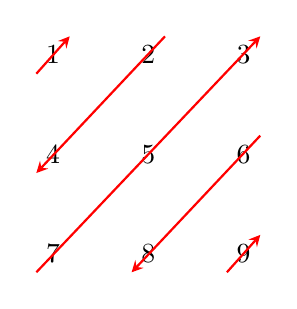
\begin{tikzpicture}
\matrix[row sep=8mm, column sep=8mm]
{
\node(1) {1}; & \node(2) {2}; & \node(3) {3}; \\
\node(4) {4}; & \node(5) {5}; & \node(6) {6}; \\
\node(7) {7}; & \node(8) {8}; & \node(9) {9};\\
};

\draw[red, thick, >=stealth, ->] (1.south west) -- (1.north east);
\draw[red, thick, >=stealth, ->] (2.north east) -- (4.south west);
\draw[red, thick, >=stealth, ->] (7.south west) -- (3.north east);
\draw[red, thick, >=stealth, ->] (6.north east) -- (8.south west);
\draw[red, thick, >=stealth, ->] (9.south west) -- (9.north east);
\end{tikzpicture}
\end{figure}
\end{flushleft}

\subsection{Matrix Trace}
在对角线上的元素的row和column index之和是相等的。

\setcounter{lstlisting}{0}
\begin{lstlisting}[style=customc, caption={Diagonal Element Has Same Sum Of Row and Column}]
vector<int> findDiagonalOrder( vector<vector<int>>& matrix )
{
    if( matrix.empty() || matrix[0].empty() )
    {
        return {};
    }

    size_t M = matrix.size();
    size_t N = matrix[0].size();

    //save the travese path
    vector<vector<int>> trace( M + N - 1 );

    for( size_t r = 0; r < M; ++r )
    {
        for( size_t c = 0; c < N; ++c )
        {
            auto x = r + c;

            trace[x].push_back( matrix[r][c] );
        }
    }

    vector<int> ans;
    ans.reserve( M + N );

    for( size_t i = 0; i < trace.size(); ++i )
    {
        if( i & 1 )
        {
            //odd sum: the direction is from top to bottom
            ans.insert( ans.end(), trace[i].begin(), trace[i].end() );
        }
        else
        {
            //even sum:  the direction is from bottom to top
            ans.insert( ans.end(), trace[i].rbegin(), trace[i].rend() );
        }
    }

    return ans;
}
\end{lstlisting}

\subsection{No Extra Memory}
\begin{itemize}
\item 有两个移动方向:向右上方移动,坐标变化为$[-1, 1]$,向左下方移动,坐标变化则为$[1, -1]$。
\item 可以根据坐标之和判断移动方向。奇数则向左下方移动,偶数向右上方移动。
\item 判断越界时,需要先判断row 或者column是否已经处于最大值的地方。因为每次越界,都要将column或者row increment。如果先判断row或者column是否为零,则会导致column或者row越界。
\end{itemize}

\setcounter{lstlisting}{0}
\begin{lstlisting}[style=customc, caption={Without Extra Memory}]
vector<int> findDiagonalOrder( vector<vector<int>>& matrix )
{
    if( matrix.empty() || matrix[0].empty() )
    {
        return {};
    }

    int M = static_cast<int>( matrix.size() );
    int N = static_cast<int>( matrix[0].size() );

    int r = 0;
    int c = 0;

    vector<int> ans( M * N );

    for( int i = 0; i < M * N; ++i )
    {

        ans[i] = matrix[r][c];

        int x = ( r + c );

        if( x & 1 )
        {
            //move down-left
            if( r == M - 1 )
            {
                //we need to check if row is in the bottom end first
                //cross boundary
                ++c;
            }
            else if( c == 0 )
            {
                //cross boundary
                ++r;
            }
            else
            {
                ++r;
                --c;
            }
        }
        else
        {
            //move up-right
            if( c == N - 1 )
            {
                //we need to check if column is at the right end first
                //cross boundary
                ++r;
            }
            else if( r == 0 )
            {
                //cross bounary
                ++c;
            }
            else
            {
                --r;
                ++c;
            }
        }
    }

    return ans;
}
\end{lstlisting}